\documentclass[a4paper,twocolumn,12pt]{article}
\usepackage{url}
\usepackage{graphicx}

\title{gmZPU SoC Datasheet}

\author{Koen Martens\\
        \texttt{kmartens@sonologic.nl}}

\begin{document}
\maketitle

\section{Introduction}

The gmZPU System-on-Chip (SoC) combines the zpu zealot medium core \cite{zpu} with two WISHBONE B4 \cite{wishbone} buses. One of the WISHBONE buses connects internal devices to the zpu. The other WISHBONE bus is exported for external devices. Figure \ref{fig:block_diagram} shows the top-level block diagram of the gmZPU SoC.

\begin{figure*}
    \centering
    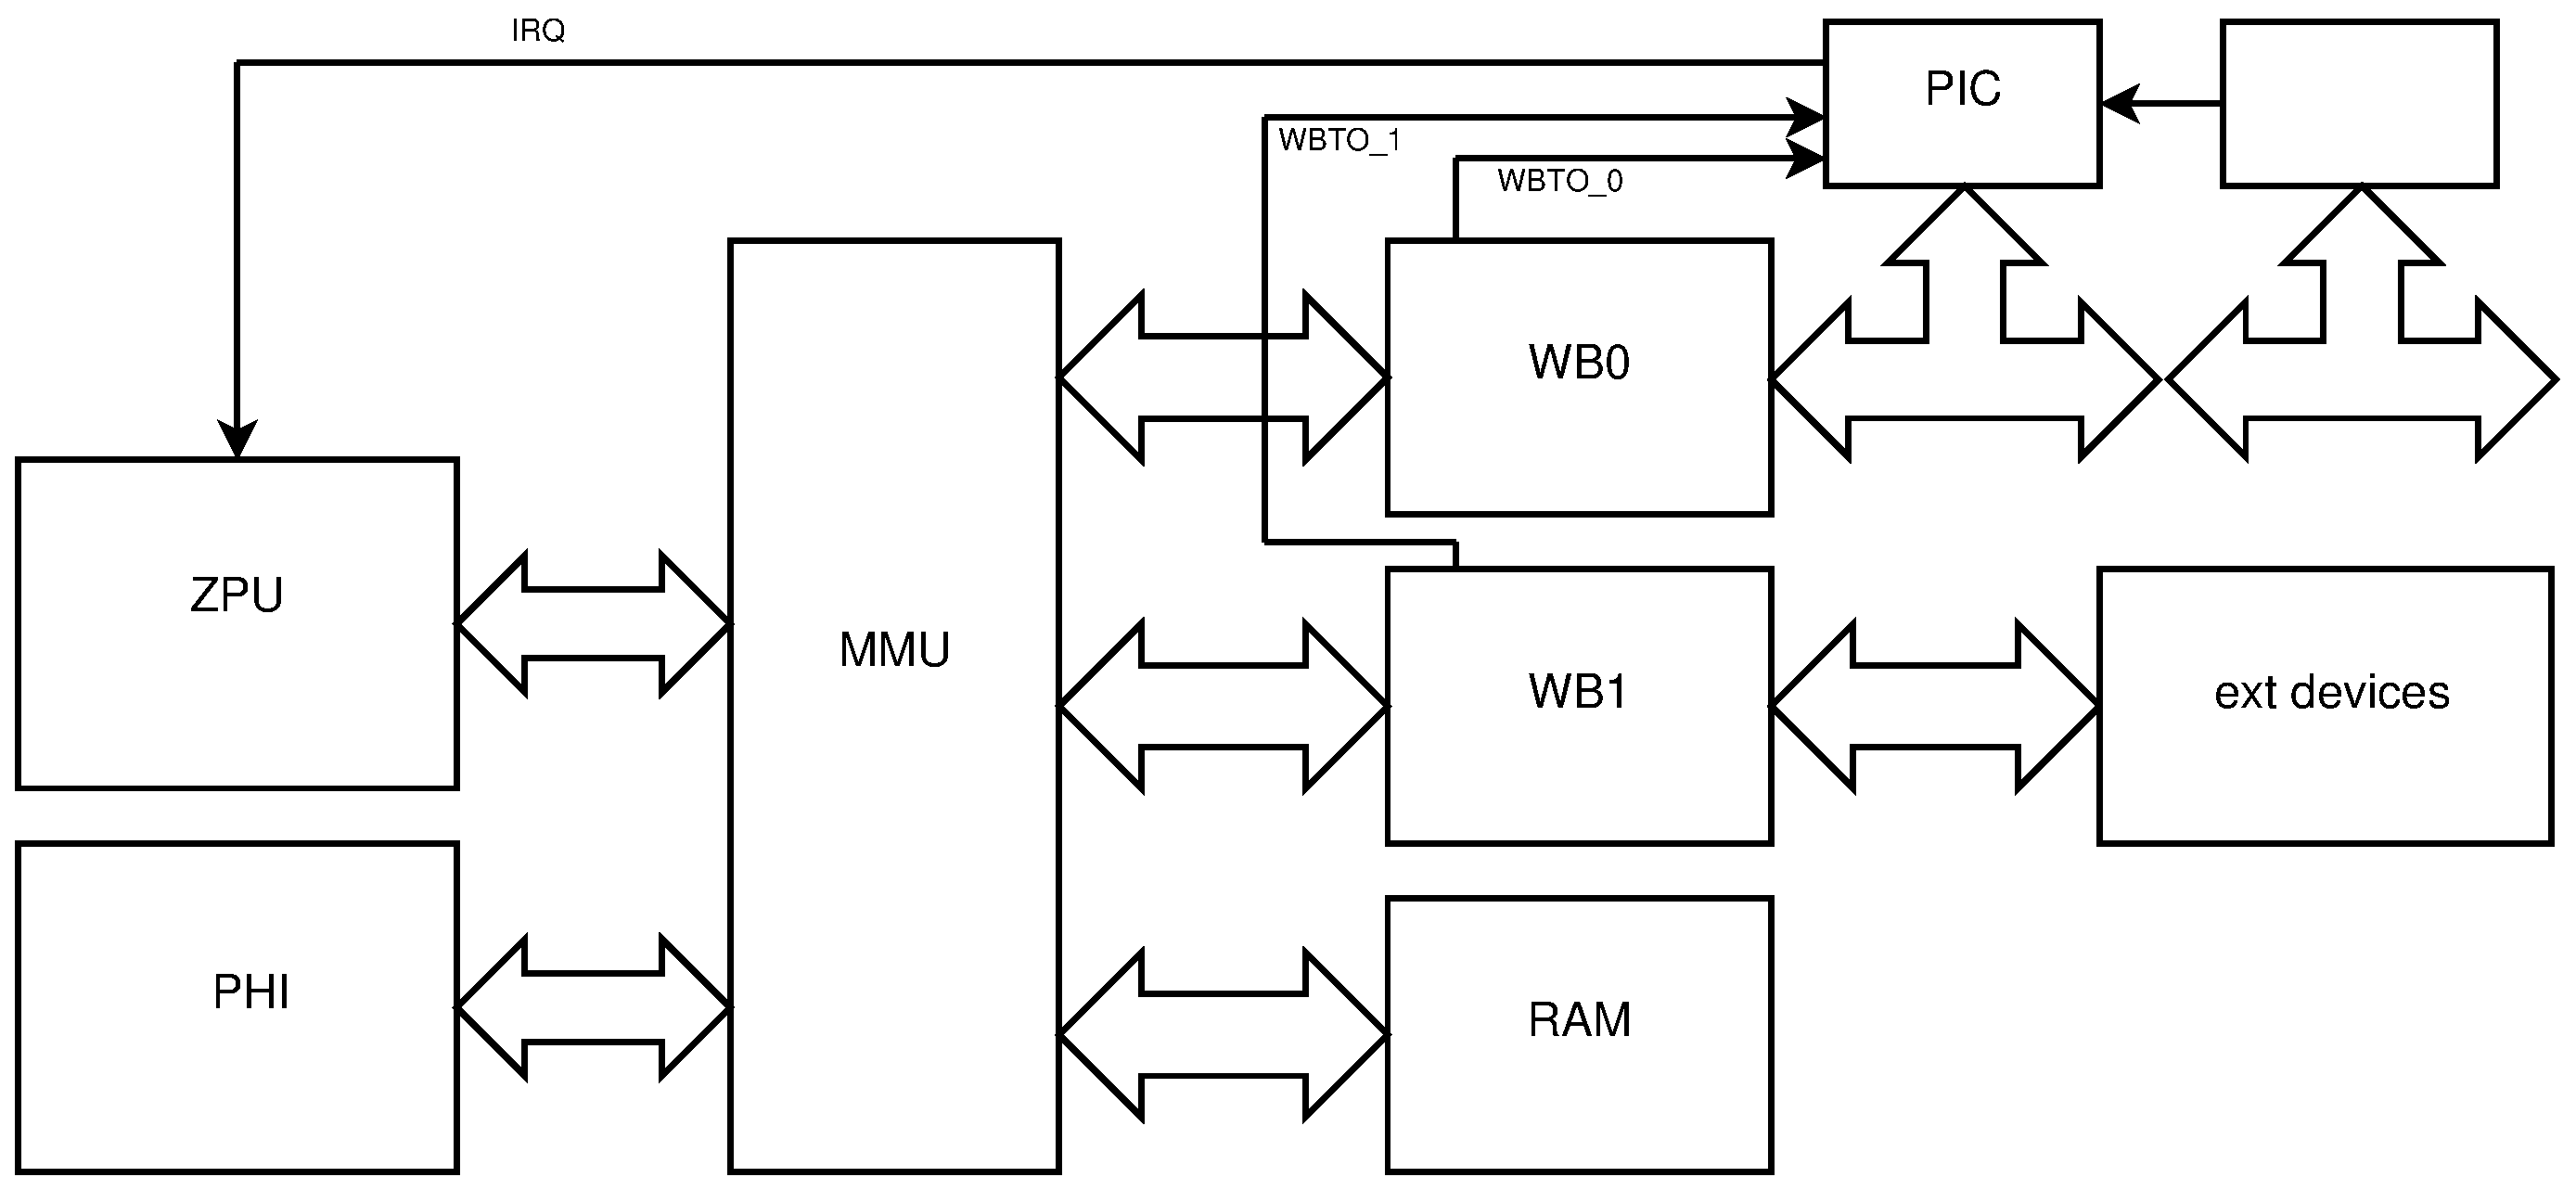
\includegraphics[width=15cm]{gmzpu_block_diagram}
    \caption{Block diagram}
    \label{fig:block_diagram}
\end{figure*}

The zpu data bus is 32 bits wide. The address bus is 18 bits wide. The Memory Management Unit (MMU) decodes the 18-bit address into chip-select and reduced address bus for the main components of the SoC interconnect fabric:

\begin{itemize}
    \item RAM
    \item phiIO basic zpu I/O
    \item WISHBONE controller 0 (WB0)
    \item WISHBONE controller 1 (WB1)
\end{itemize}

\section{Notation}

\begin{description}
    \item[BUS(1:0)] Bit 1 downto 0 of bus BUS.
\end{description}

\section{Memory map}

The 8 most significant bits of the zpu address bus select one of the core components linked directly to the zpu. Table \ref{tab:address_bits} shows how these bits are decoded.

\begin{table}[h]
\caption{Address decoding}
\label{tab:address_bits}
\begin{tabular}{| c | c | c | c | c | c | c | c | l |
}
    \hline
    17 & 16 & 15 & 14 & 13 & 12 & 11 & 10 & chip select \\ \hline
    0  & X  & X  & X  & X  & X  & X  & X  & RAM \\ \hline
    1  & 0  & X  & X  & X  & X  & X  & X  & phiIO \\ \hline
    1  & 1  & 0  & X  & X  & X  & X  & X  & WB0 control \\ \hline
    1  & 1  & 1  & 0  & 0  & 0  & 0  & X  & WB0 slave 0 \\ \hline
    1  & 1  & 1  & 0  & 0  & 0  & 1  & X  & WB0 slave 1 \\ \hline
\end{tabular}
\end{table}

Each core component has a specific address bus width. Table \ref{tab:address_map_hex} shows the base address of each of the core components shown in \ref{tab:address_bits}. Along with the base address is the size of the address bus to that device.

\begin{table}[h]
\caption{Address map and sizes}
\label{tab:address_map_hex}
\begin{tabular}{| l | c | c | c |
}
    \hline
    Device      & Base    & Size    & Bytes \\ \hline
    RAM         & 0x00000 & 0x20000 & 128k  \\ \hline
    phIO        & 0x20000 & 0x10000 & 64k   \\ \hline
    WB0 control & 0x30000 & 0x08000 & 32K   \\ \hline
    WB0 slave 0 & 0x38000 & 0x00800 & 2K    \\ \hline
    WB0 slave 1 & 0x38800 & 0x00800 & 2k    \\ \hline
\end{tabular}
\end{table}

\section{Internal devices}

 Lorem ipsum dolor sit amet, consectetur adipiscing elit. Vestibulum tempor ipsum sit amet mauris ornare, eget tincidunt mauris bibendum. Phasellus tincidunt vulputate dignissim. Suspendisse blandit aliquam ante, at commodo diam tincidunt sit amet. Donec ut scelerisque mi. Proin ipsum justo, convallis vitae ante ut, porta bibendum nunc. Nunc nisi turpis, tincidunt non lorem eu, euismod dignissim tellus. Mauris suscipit, augue quis eleifend tristique, libero eros molestie orci, vitae pretium ipsum metus vel dui. Nullam condimentum, est vel congue lacinia, tellus tortor vestibulum neque, vel pulvinar neque orci non odio.

Donec tempor risus orci, vel sodales turpis mattis sit amet. Nullam elementum adipiscing nulla, sed commodo purus posuere id. Donec sollicitudin ullamcorper interdum. Praesent ultrices et lacus a condimentum. Curabitur porttitor, libero in tristique aliquam, enim leo rutrum metus, vel interdum nisi ligula vel libero. Duis hendrerit urna scelerisque nulla convallis facilisis. Maecenas in tellus orci. Duis ante metus, mollis a ligula non, aliquet tempor leo. Donec at ante mauris.

Maecenas lobortis vulputate lobortis. Nunc pulvinar convallis tortor eu luctus. Sed vehicula ipsum a neque dictum, sed ornare dolor luctus. Curabitur hendrerit dui et ante rhoncus vulputate. Curabitur a nibh ultricies, ornare eros sit amet, pharetra sapien. Vestibulum venenatis convallis feugiat. Nulla leo turpis, facilisis vitae velit ac, dignissim blandit quam. Sed vehicula metus sit amet imperdiet ullamcorper. Etiam eget cursus orci, vitae ultrices est. Vivamus ac quam tincidunt, porta orci at, vehicula mi. Integer eros massa, egestas vitae facilisis eleifend, iaculis auctor ligula. 

\subsection{Programmable Interrupt Controller (PIC)}

Donec non pulvinar sem. Mauris elementum euismod vulputate. In a pretium massa. Quisque lacus enim, euismod ut dapibus sed, pretium at purus. Etiam eu massa erat. Nam semper, arcu eu mollis euismod, tellus lacus scelerisque ligula, in cursus orci quam eu odio. Vivamus tincidunt consectetur neque a tempus. Lorem ipsum dolor sit amet, consectetur adipiscing elit. Suspendisse velit lorem, consequat in sapien in, vulputate cursus nisl. Aenean rutrum nisi eu ligula vulputate vulputate. Pellentesque habitant morbi tristique senectus et netus et malesuada fames ac turpis egestas. Vivamus risus tortor, imperdiet et sollicitudin convallis, ultricies interdum massa. Sed volutpat enim id mauris facilisis rhoncus.

Donec molestie fermentum sodales. Ut pellentesque dolor non nulla commodo dignissim. Etiam nec porta est, a porta odio. Nam eu fermentum metus. Ut elit libero, porttitor ac lacus ac, ornare tempus lacus. Cras ac ultricies nisi. Nunc porttitor massa non erat blandit dapibus. In hac habitasse platea dictumst. In hac habitasse platea dictumst. Praesent ac aliquet quam. Cras mattis lectus et metus laoreet fringilla. Donec viverra sem at iaculis lacinia. Integer lorem augue, aliquet vel fringilla eget, consectetur malesuada lorem. Cras quis tortor vitae lacus fermentum bibendum id nec diam. Curabitur tempus, turpis ac cursus pretium, augue metus commodo nisi, non hendrerit mi justo eu nisl. 

\begin{thebibliography}{9}

\bibitem{wishbone} OpenCores \emph{Wishbone B4, WISHBONE System-on-Chip (SoC)Interconnection Architecture for Portable IP Cores} \url{http://opencores.org/opencores,wishbone} 2010.

\bibitem{zpu} Zylin Consulting \emph{Zylin ZPU} \url{http://opensource.zylin.com/zpu.htm}.

\bibitem{gmzpu} Sonologic \emph{gmzpu github repository} \url{http://github.com/sonologic/gmzpu}.

\end{thebibliography}

\end{document}

